\documentclass[tikz,border=10pt]{standalone}

\begin{document}
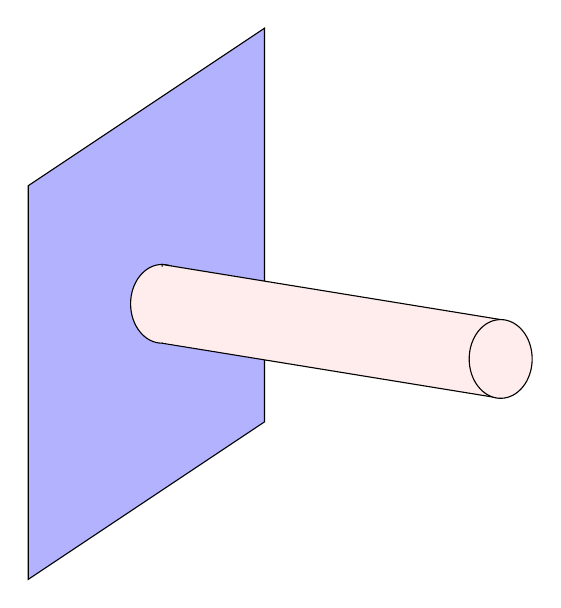
\begin{tikzpicture}
    % Draw the filled polygon
    \filldraw[fill=blue!30] (0,-2) -- (3,0) -- (3,-5) -- (0,-7) -- cycle;
    
    % Draw the first ellipse
    \filldraw[fill=pink!30] (1.7,-3.5) ellipse (0.4 and 0.5); % Width is 0.8 of height, so if height = 1, width = 0.8
    \filldraw[fill=pink!30] (1.7,-3.5+0.5) -- (6,-4.2+0.5) -- (6,-4.2-0.5) -- (1.7,-3.5-0.5) -- cycle;
    % Draw the second ellipse
    \filldraw[fill=pink!30] (6,-4.2) ellipse (0.4 and 0.5); % Same dimensions as the first ellipse

    % Draw the connecting rectangle (represents the body of the cylinder)
    \fill[pink!30] (1.65,-3.5+0.48) -- (5,-4.2+0.48) -- (5,-4.2-0.31) -- (1.65,-3.5-0.48) -- cycle;

\end{tikzpicture}
\end{document}
